\section{Introduction}
\label{s:Introduction}
This report will guide you through the work done in the past six months at the Harvard Micro-robotics Lab. 

Soft robotics are a developing field in  the world of automated devices. In most of the cases conventional robots are composed of rigid links  and supported by an algorithm based on the physical model to create predictable movements. These properties are very useful especially in industrial setups such as the automotive industry. With proper control repeatable tasks can be fulfilled with high precision and safety (using safeguards).  Soft-robots though,  are defined as having a reduced to low rigidity body and show flexibility and compliance with the environment and the objects they interact with. Stresses caused from any contact will first make the robot yield and comply before causing any significant damage to the target e.g., living organisms and humans. \cite{trivedi2008soft, rus2015design, polygerinos2017soft}. Therefore they can give a user a certain confidence when it comes to fulfilling a mission with low to null damage. Their rather simplified control adds to their usability, and a potential larger range of use cases. Without any wordplay, this feature makes them very flexible.

\subsection{Inspiration}
\label{s:Inspiration}
As humans we often want to mimic and reproduce phenomena we observe in nature. We especially focus on those we think will improve our lives and seek inspiration in all kinds of living creatures that surround us, from the deep seas to the rain-forests. 
Inspiration in soft-robotics is mainly biological and comes from animals like cephalopods (see Figure~\ref{f:Inspiration}), jellyfish or humans themselves. Even particular parts of the bodies are of specific interest such as elephant trunks (see Figure~\ref{f:Inspiration}\footnote{Pinterest: https://www.pinterest.ch/pin/345510602657383002/}) or the human tongue which are hydrostatic muscles. They rely on the incompressible property of water to actuate themselves. Through muscular cells and fibers they form elongated soft structures that are very adaptable (taking various shapes and positions). They can go through various elongations, bending and torsion modes. The octopus is a good example of a fully soft organism with no rigid skeleton. Composed of eight arms around a head, it is able to change itself to fit the environment and go through various holes and complicated mazes\footnote{National Georgraphic: https://youtu.be/SCAIedFgdY0}. Squids on the other hand have a few rigid cartilages supporting their body in an elongated nose cone-like shape allowing them to move fast in water.Though both are still molluscs (invertebrate). The same analogy can be done in soft robotics where different applications require a variety of compliance and stiffness properties thanks to inner or outer structures including links, plates or rods.

\begin{figure}[ht]
\centering
\subfigure[Pair of cuttlefish]{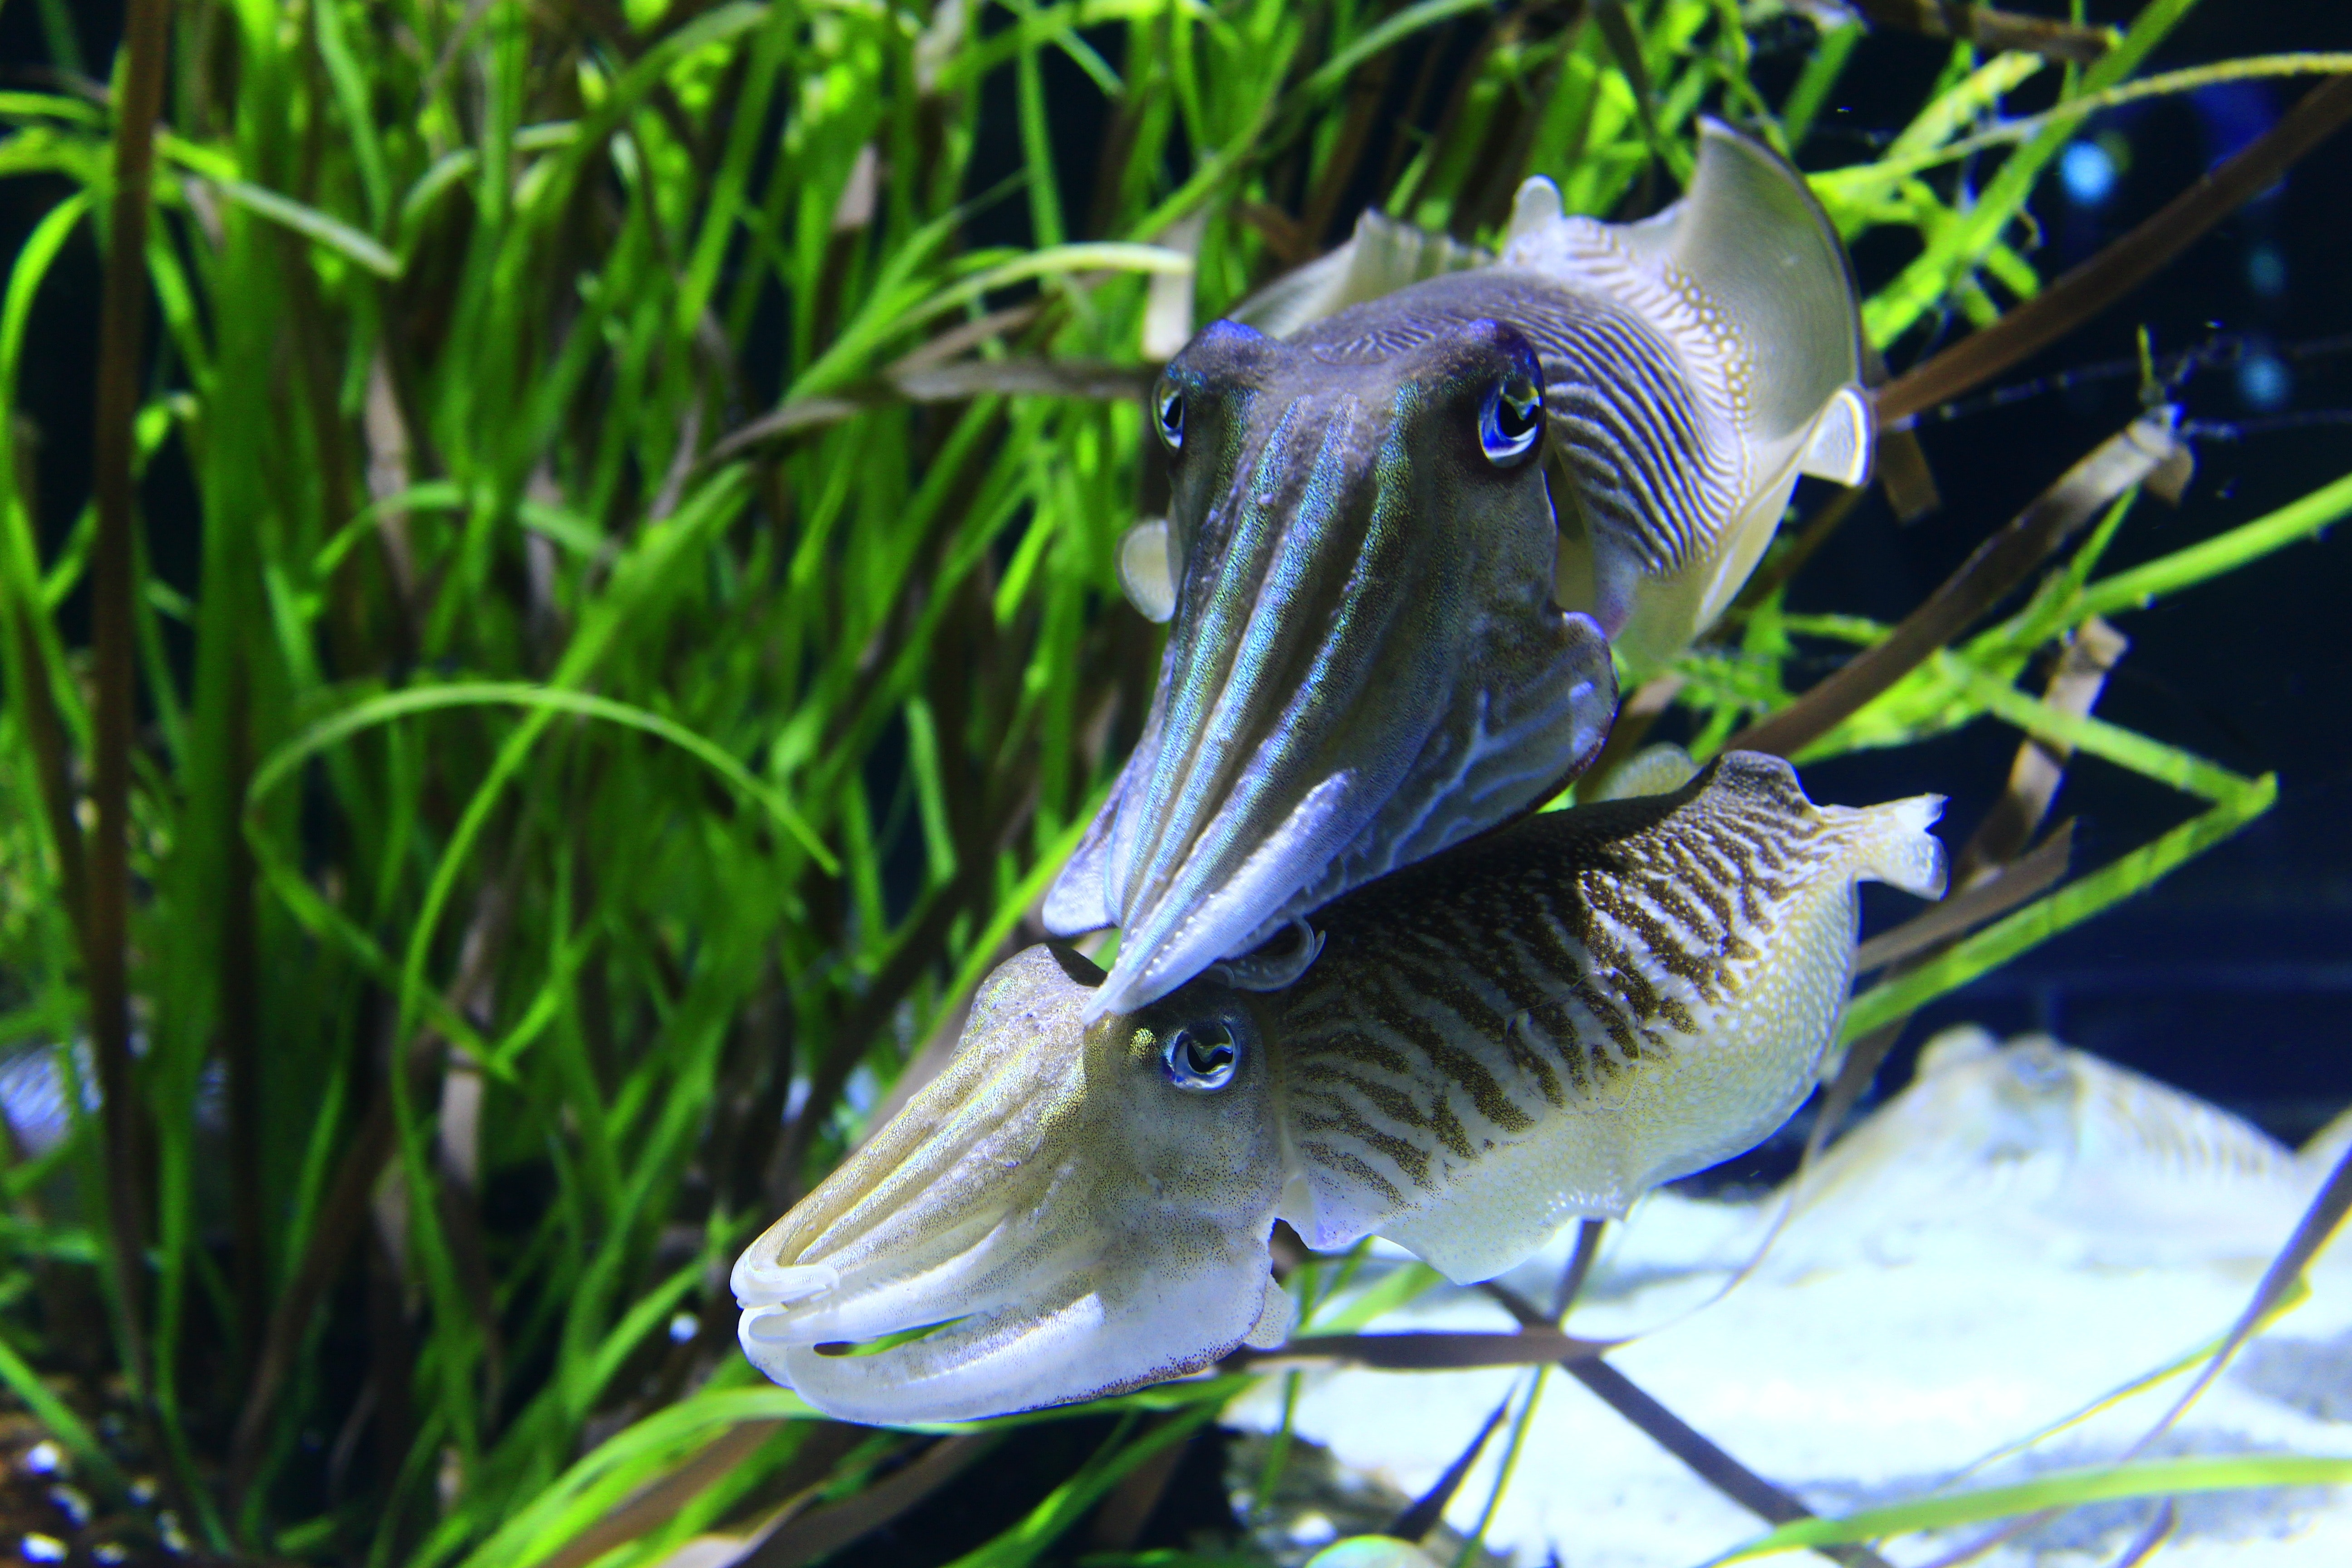
\includegraphics[height=50mm]{Images/cuttlefish.jpg}}\quad
\subfigure[Elephant trunk]{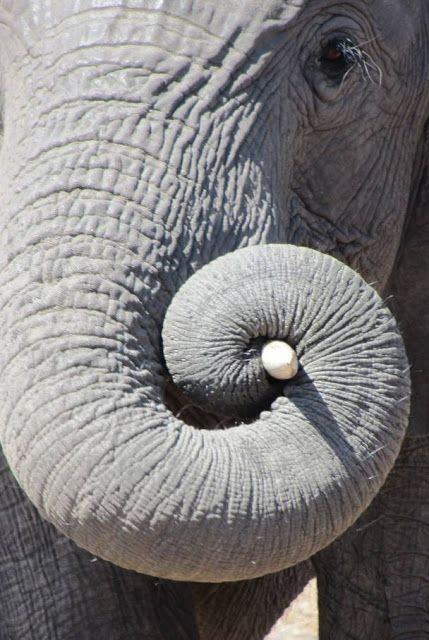
\includegraphics[height=50mm]{Images/elephant_trunk.jpg}}
\caption[Inspiration]{\label{f:Inspiration}(a) Cuttlefish are cephalopods with a rigid backbone.(b) A curled elephant trunk is a good example of a muscular hydrostat.}
\end{figure}


\subsection{Application}
\label{s:Application}
Soft robotic applications are very broad, the focus is , though,  mainly set on interactions with fragile and sensitive objects or living organisms (humans included). Even though common robots do perform very well (in medicine : da Vinci \footnote{da Vinci: https://www.intuitive.com/}), they are often very expensive and complex \cite{polygerinos2017soft}. Due to a similar impedance soft-robots reduce destructive contact forces allowing a safer manipulation. However this characteristic comes with a trade-off: the softer the robot the more difficult it is to manage its shape and  movements without reintroducing rigid parts. It involves combining the right materials \cite{polygerinos2017soft} with the right actuation making the whole structure intelligent \cite{rus2015design}. Some are specially designed for surgical purpose such as catheters or implantable devices \cite{levering2014soft, polygerinos2017soft}, and are meant to avoid critical damage to be done to tissues and other organs when operating. Others are used as wearable devices either for rehabilitation purposes or enhancing the body's capabilities by using for instance muscle-like actuation \cite{park2014design, polygerinos2017soft}. We also find soft-robots in deep-sea exploration. The main reason being that at high depths, fragile animals and living organisms might be encountered very rarely and as to preserve their integrity a gentle approach is required \cite{Galloway2016, Kurumaya2018}.

\subsection{Motivation}
\label{s:Motivation}
If unexpected changes occur in the environment, is there a possibility to adapt to it and react accordingly by adjusting the stiffness of the fingers? This particular feature would allow modifying on the fly the range of potential target objects and not bother about using a complete different hand.

In this work we will try to improve the grasping range of a soft robotic hand for deep-sea exploration by bringing a variable stiffness feature to every single finger. Through a vision based measurement system characterization of single fingers will be possible. Thanks to a benchmarking method we will also compare the different designs. Those methods should be made in a generalized way so as to be applicable to other soft robotic manipulators as well as rigid ones in order to compare them on a similar and standardized basis.

The gripper we are using for now has been classified as a controlled actuation gripper by Shintake and Cacucciolo \cite{shintake2018soft}. One goal would be to show a possible combination of simple actuation and controlled stiffness in a single finger and develop a possible method to do so. Different possibilities are offered to us such as the use of jamming, or multi-channel pressure chambers embedded inside the finger as well as guidance wires. 


